\chapter{Viabilidade financeira}

No âmbito do desenvolvimento de uma aplicação, a avaliação de sua viabilidade financeira assume um papel de extrema importância, exercendo influência significativa na análise de projetos e na formulação de decisões estratégicas. A primordialidade deste aspecto se funda na sua capacidade de assegurar uma avaliação meticulosa dos encargos associados e uma projeção pragmática das receitas projetadas, ambas essenciais para garantir a sustentabilidade do projeto e a concretização de um retorno financeiro condizente com os objetivos almejados.

% Estimativas
\section{Estimativas de usuários}

Esta seção tem como objetivo traçar uma estimativa dos possíveis usuários da plataforma desenvolvida, com o intuito de fornecer embasamento aos cálculos para realizar as previsões financeiras.

\subsection{Aplicações com público-alvo semelhantes}\label{subsec::publico-alvo_semelhante}

Neste tópico, serão analisadas as plataformas que possuem um público-alvo semelhante ao da \textit{GameLocker}. O objetivo da análise é alcançar um valor equilibrado para a assinatura \textit{premium} do sistema e realizar uma estimativa geral dos usuários que podem ser alcançados, levando em consideração a proporção de uma plataforma recém-lançada.

\subsubsection{Discord}

A plataforma \textit{\gls{Discord}} engloba chamadas de voz, mensagens escritas e uma gama variada de recursos para seus usuários. Conforme citado por Ash Turner \cite{discord_users}, aproximadamente 70\% dos usuários da plataforma a utilizam para jogar \textit{videogame} e outras atividades, como grupos de estudos. Essa informação leva à conclusão de que o público-alvo desse sistema se assemelha ao da \textit{GameLocker}.

De acordo com informações disponíveis no site oficial do \textit{\gls{Discord}} (Disponível em: \url{https://discord.com/nitro}), a plataforma oferece uma opção de assinatura mensal ao custo de \textit{R\$ 25,00}. Essa assinatura proporciona aos utilizadores a expansão da capacidade de \textit{uploads} de arquivos, uma personalização mais profunda de perfis, bem como a capacidade de transmitir vídeos em alta definição (HD), entre outros benefícios de significativa relevância.

\subsubsection{Twitch}

A \textit{\gls{Twitch}}, atualmente, desempenha um papel de destaque como uma das mais renomadas plataformas de transmissão em tempo real global. Conforme apontado pela VentureBeat \cite{twitch_categories}, nove das dez categorias mais assistidas na \textit{\gls{Twitch}} estão relacionadas a jogos eletrônicos, mantendo-se constantemente em evidência e atraindo diariamente centenas de milhares de espectadores. Essa dinâmica a torna um espaço amplamente explorado pelo público-alvo que este projeto busca alcançar.

De acordo com informações disponíveis em seu site oficial \url{https://www.twitch.tv}, a plataforma oferece uma opção de assinatura mensal com um custo de \textit{R\$ 26,99}. Através dessa assinatura, os usuários podem desfrutar da visualização de conteúdo livre de anúncios indesejados e têm acesso a um conjunto diversificado de recursos destinados à personalização de seus perfis. Isso inclui a utilização de \textit{emotes} personalizados, a variação de paletas de cores e a obtenção de distintivos especiais, contribuindo assim para uma experiência mais envolvente e individualizada.

\subsubsection{Estratégias de Utilização}

Este tópico visa investigar e analisar as estratégias que transformaram o \textit{\gls{Discord}} e o \textit{\gls{Twitch}} em líderes na arena da comunicação online, transcendo as suas origens como plataformas voltadas para jogos. Além disso, serão apresentadas estatísticas relacionadas ao uso e à receita dessas plataformas.

\subsubsubsection{Plano de Aplicação}

O \textit{\gls{Discord}}, desde a sua introdução em 2015, tem percorrido uma notável trajetória de evolução e adaptação, culminando na redefinição de sua imagem inicial, que estava originalmente vinculada a uma plataforma exclusivamente voltada para jogos.

\begin{itemize}
    \item \textbf{Diversificação de Servidores}: Servidores dedicados a jogos, permitindo que os jogadores se reunissem em um ambiente específico para cada jogo;
    \item \textbf{Expansão para Além dos Jogos}: Embora tenha começado como uma plataforma de jogos, o \textit{\gls{Discord}} expandiu sua base de usuários para incluir não jogadores, competindo com ferramentas de comunicação empresarial como \textit{Slack} e \textit{Microsoft Teams};
    \item \textbf{Combate à Controvérsia}: O \textit{\gls{Discord}} enfrentou desafios, incluindo a controvérsia em torno do uso de servidores privados por grupos extremistas. A empresa implementou ferramentas de moderação e verificação para lidar com esses problemas, destacando seu compromisso com a segurança e responsabilidade.
\end{itemize}

A \textit{\gls{Twitch}}, uma plataforma líder de comunicação, tem expandido significativamente seu escopo muito além de sua imagem inicial, que estava predominantemente associada à transmissão de jogos.

\begin{itemize}
    \item \textbf{Diversificação de Conteúdo}: Embora o \textit{\gls{Twitch}} seja amplamente associado à transmissão de jogos, a plataforma diversificou seu conteúdo ao longo do tempo. Além das transmissões de jogos, os criadores agora utilizam o \textit{Just Chatting} e outras categorias para transmitir uma variedade de conteúdos, como shows ao vivo, música e arte;
    \item \textbf{Parcerias e Integrações}: Estabelecer parcerias estratégicas com empresas e criadores de conteúdo, o que ajudou a atrair um público diversificado. Além disso, integrações com plataformas como \textit{\gls{Amazon Prime}} e eventos como o \textit{TwitchCon} fortaleceram a presença da plataforma;
    \item \textbf{Monetização para Criadores}: Introduzir maneiras inovadoras de monetização para criadores, como assinaturas de canais, doações e anúncios. Essas estratégias tornaram possível que criadores ganhassem renda significativa transmitindo seu conteúdo na plataforma.
\end{itemize}

\subsubsubsection{Estatísticas de Uso e Receita}

A \textit{\gls{Twitch}} registra 140 milhões de usuários ativos mensais, demonstrando sua extensa popularidade. Essa estatística por si só destaca a importância da plataforma no cenário de entretenimento online. Conforme apontado pela Backlink \cite{twitch_growth_statistics} e descrito na Figura \ref{crescimentoUsoTwitch}.

\begin{figure}[H]
    \center
	\caption{\label{fig_sge20}Crescimento do Uso da Twitch}
    \label{crescimentoUsoTwitch}
    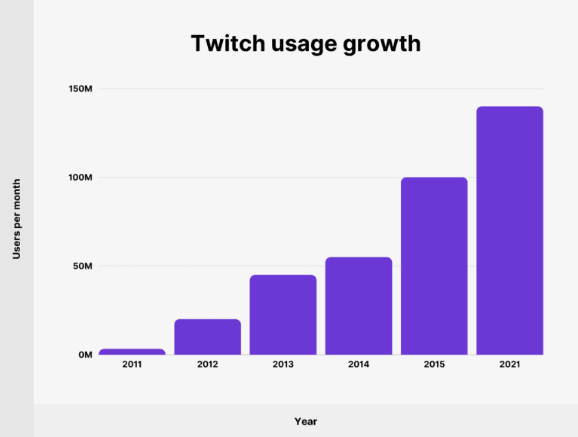
\includegraphics[scale=0.85]{imagens/viabilidadeFinanceira/CrescimentoTwitch.png}
	\fonte{\cite{twitch_growth_statistics}}
\end{figure}

Com 7,4 milhões de \textit{streamers} criando conteúdo a cada mês e um total de 9,2 milhões de \textit{streamers} ativos, fica claro que a comunidade de criadores desempenha um papel fundamental na expansão do \textit{\gls{Twitch}}. Os espectadores do \textit{\gls{Twitch}} assistem coletivamente a uma incrível quantidade de conteúdo, totalizando 1,14 trilhão de minutos assistidos, equivalentes a 1,86 bilhão de horas mensais.

Em termos de receita anual de publicidade, o \textit{\gls{Twitch}} alcançou a marca de US\$ 231,8 milhões, representando mais que o dobro dos US\$ 102,5 milhões registrados em 2017. Além da publicidade, outra fonte significativa de receita para o \textit{\gls{Twitch}} é o sistema de assinaturas. No entanto, a avaliação precisa dessa receita é desafiadora, uma vez que as assinaturas \textit{premium} do \textit{\gls{Amazon Prime}} incluem automaticamente a assinatura \textit{premium} do \textit{\gls{Twitch}}. Estimativas indicam que a receita anual total do \textit{\gls{Twitch}} gira em torno de US\$ 1,54 bilhão.

No que tange à base de usuários, o \textit{\gls{Discord}} ostenta números notáveis, com uma marca impressionante de 140 milhões de usuários ativos mensais, conforme demonstra a Figura \ref{usuariosMensaisDiscord}. Mais notável ainda é o fato de que essa base dobrou no último ano, o que atesta um crescimento substancial e sustentado ao longo do tempo. 

\begin{figure}[H]
    \center
	\caption{\label{fig_sge20}Usuários ativos mensais do Discord}
    \label{usuariosMensaisDiscord}
    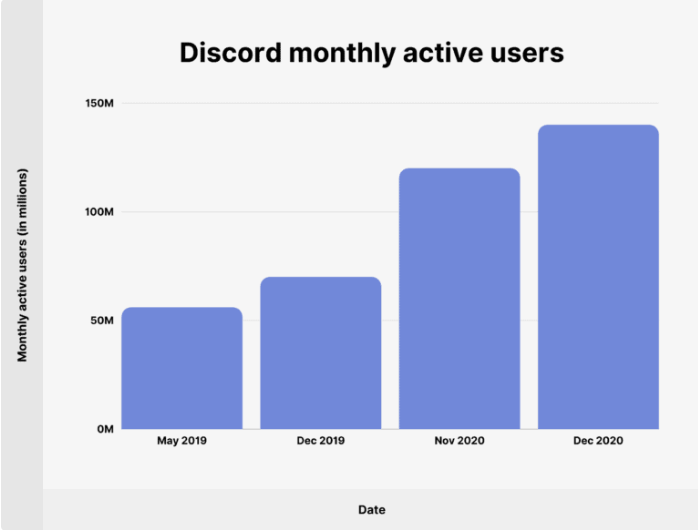
\includegraphics[scale=0.7]{imagens/viabilidadeFinanceira/DiscordActiveUsers.png}
	\fonte{\cite{discord_active_users}}
\end{figure}

No âmbito dos investimentos, o \textit{\gls{Discord}} angariou uma expressiva quantia de financiamento, totalizando US\$ 483,8 milhões. Além disso, o \textit{\gls{Discord}} demonstra sua capacidade de monetização ao gerar uma receita anual considerável, totalizando US\$ 130 milhões. Com uma valoração atual de US\$ 7 bilhões e uma rede de cerca de 13,5 milhões de servidores ativos por semana, o \textit{\gls{Discord}} emerge como um protagonista fundamental no cenário das interações online, consolidando-se como uma das principais plataformas de comunicação no mundo.

\subsection{Análise e Projeção}

Para estimar o crescimento de usuários do projeto, foi adotada como abordagem de análise uma curva normal de crescimento. Estabelecemos como meta de projeção um incremento de 1\% no número de usuários ativos em relação às duas plataformas mencionadas, ao término dos primeiros 12 meses.

A projeção de um aumento de 1\% ao longo do período de 12 meses resultaria em um total de 30.000 usuários ativos na plataforma. Ressalta-se a relevância deste crescimento gradual, o qual segue uma trajetória ascendente que se alinha com as tendências observadas na \textit{\gls{Twitch}} e no \textit{\gls{Discord}}. Cabe destacar que, embora o projeto esteja em estágio inicial e não disponha da mesma base de usuários das plataformas mencionadas, a tendência de crescimento sustentado é promissora.

Com base nas informações disponíveis sobre a \textit{\gls{Twitch}} e o \textit{\gls{Discord}}, é plenamente justificável projetar um aumento gradual para o presente projeto. As referidas plataformas representam notáveis exemplos de sucesso no âmbito do entretenimento online e da comunicação, o que reflete a crescente demanda por tais serviços. Nesse contexto, a estimativa de crescimento de usuários apresentada neste estudo está fundamentada em bases sólidas e aponta para um considerável potencial.

% Despesas
\section{Despesas}

As despesas inerentes ao presente projeto encontram-se intrincadamente associadas a três fontes de destaque, nomeadamente: infraestrutura, recursos humanos e angariação de clientes.

\subsection{Infraestrutura}

Os ônus relativos à infraestrutura do projeto serão integralmente derivados dos serviços providos pela plataforma \textit{\gls{Azure}}, visto que as demais instâncias participantes se pautam pela isenção de custos. A delimitação do preço desses serviços foi efetuada por intermédio da aplicação da Calculadora de Custos \textit{\gls{AzurePricingCalculator}}. Nesse processo de cálculo, foram criteriosamente incorporados os serviços de \textit{\gls{AppService}} e \textit{\gls{AzureSQLDatabase}}, a fim de mensurar com precisão os dispêndios vinculados a tais soluções. A tabela \ref{estimativaAzure} elucida a projeção orçamentária referente à Azure.

\begin{table}[H]
    \setcounter{table}{0}
    \center
	\caption{Custos Azure Services}
    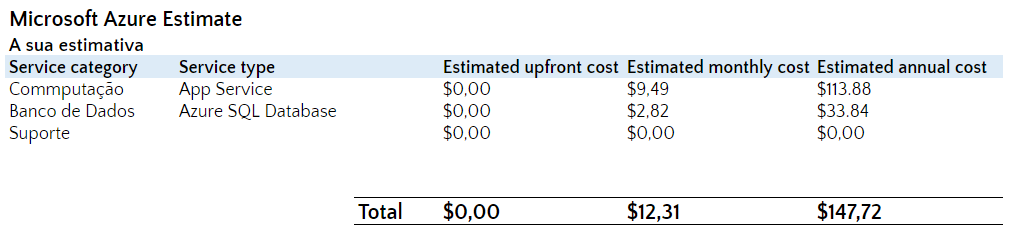
\includegraphics[scale=0.55]{imagens/viabilidadeFinanceira/estimativaAzure.png}
    \label{estimativaAzure}
	\fonte{Azure Pricing Calculator}
\end{table}

De acordo com a estimativa de usuários realizada, foi possível estimar também os custos de infraestrutura gerados, fornecendo uma visualização dessa fonte de despesas, como pode ser visto na tabela \ref{estimativaAzure}.

\subsection{Recursos Humanos}

No contexto de um projeto no âmbito da tecnologia, a apropriação dos recursos financeiros destinados aos elementos humanos compreende uma amplitude abrangente de fatores mutuamente interligados. Estes englobam componentes como a remuneração dos colaboradores, as obrigações fiscais e previdenciárias, as vantagens e benefícios oferecidos, as iniciativas de aperfeiçoamento e o contínuo desenvolvimento profissional. A competente gestão desses recursos assume um papel preponderante, exercendo uma influência crucial no sucesso do empreendimento e na maximização dos aportes investidos.

No que tange às remunerações, os desembolsos podem variar significativamente devido às posições ocupadas e ao nível de especialização dos membros da equipe. Os encargos trabalhistas, abarcando as contribuições sociais e outras obrigações jurídicas, também compõem a soma total dedicada.

A concessão de benefícios, como planos de saúde, auxílios-alimentação e transporte, se converte em um elemento adicional, conferindo um acréscimo financeiro ao montante designado. A capacitação da equipe, mediante a implementação de programas de formação e atualização, insere-se no âmbito do investimento, salvaguardando a manutenção da excelência laboral em um cenário tecnológico em constante mutação.

De acordo com as orientações preconizadas por plataformas especializadas em oportunidades de trabalho, análises de mercado e organizações dedicadas ao recrutamento, os valores correspondentes às despesas podem ser delineados com base em uma média geral:

\begin{itemize}
    \item \textbf{Salário de Estágio}: R\$ 1.500,00;
    \item \textbf{Encargos Trabalhistas (aproximadamente 70\% do salário)}: R\$ 1.050,00;
    \item \textbf{Benefícios (plano de saúde, vale-transporte, vale-alimentação)}: R\$ 300,00.
\end{itemize}

Considerando que a configuração da equipe é constituída por um grupo de seis desenvolvedores em nível de estágio, os montantes financeiros mensais que imperam no cenário comercial foram incorporados à análise, conforme o Quadro \ref{despesasRecursosHumanos}:

\begin{itemize}
    \item Custo base: R\$ 2.800,00
    \item Dias-base: 22 | Dia-hora: 8
    \item Custo-hora: R\$ 15,90
\end{itemize}

\begin{quadro}[H]
\centering
\caption{Despesas dos Recursos Humanos}
\label{despesasRecursosHumanos}
\begin{longtable}{|p{5cm}|p{3cm}|p{3cm}|}
\hline
Despesa & 6 meses & 12 meses
\\\hline
Salário & R\$ 54.000,00 & R\$ 108.000,00\
\\\hline
Encargos Trabalhistas & R\$ 37.800,00 & R\$ 75.600,00\
\\\hline
Benefícios & R\$ 10.800,00 & R\$ 21.600,00\
\\\hline
\end{longtable}
\fonte{Os Autores.}
\end{quadro}

A contabilização das horas referentes ao projeto incorporou a análise de três distintas classificações de requisitos funcionais a serem incorporados: níveis fácil, médio e difícil, organizados em conformidade com a proficiência dos membros da equipe.

Para os requisitos funcionais fáceis, foi tomado como base um tempo de 48 horas de desenvolvimento. Já para os médios foi considerado o tempo de 80 horas de desenvolvimento e, para os difíceis, 160 horas. Tais despesas desempenham um papel preponderante especialmente ao longo da fase de desenvolvimento do projeto. A representação gráfica \ref{maoDeObra} evidencia a apresentação destes cálculos.

\begin{table}[H]
    \center
    \setcounter{table}{1}
	\caption{Mão de Obra Mensal}
    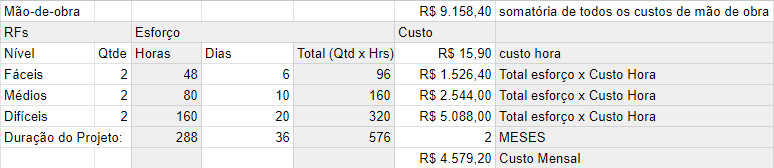
\includegraphics[scale=0.75]{imagens/viabilidadeFinanceira/MaoDeObra.png}
    \label{maoDeObra}
	\fonte{Os autores}
    \setcounter{table}{2}
\end{table}

A tabela \ref{maoDeObra} demonstra a quantidade de horas totais a serem utilizadas no projeto, bem como os custos totais com mão de obra e os custos mensais a serem assumidos. De acordo com o cálculo de horas realizado na tabela, é possível observar que a duração será de 2 meses.

\subsection{Captação de Clientes}

Com vistas a consolidar a estratégia de aquisição de clientes para a plataforma, almeja-se direcionar recursos para atividades de marketing. Isso se concretizará mediante a veiculação de anúncios em plataformas conexas ao público-alvo do projeto, a exemplo do \textit{\gls{Youtube}}, \textit{\gls{Twitch}} e \textit{\gls{Tiktok}}. A ênfase recairá na promoção desses anúncios em conteúdos especialmente voltados ao universo dos jogos eletrônicos, visando estabelecer uma afinidade precisa e maximizar a eficácia das iniciativas na atração de novos usuários para a \textit{GameLocker}.

Ademais, uma possibilidade viável consiste na divulgação nestas plataformas mediante um enfoque mais personalizado, alcançado por meio do estabelecimento de colaborações diretas com os criadores de conteúdo. A concretização destas parcerias seria intermediada por acordos de patrocínio, nos quais eles divulgariam o sistema perante sua audiência.

Dentro do contexto de cada uma das mencionadas plataformas, que permitem valores personalizados de investimento em marketing, estima-se, em um primeiro momento, um aporte de investimento mensal equivalente a R\$ 267,00, culminando, assim, em um montante total de R\$ 800,00 mensais destinado à angariação de novos usuários. Estes valores têm o objetivo de manter a captação de usuários ativa sem que o projeto se torne inviável financeiramente.

% Receitas
\section{Receitas}

Visando assegurar a viabilidade financeira do projeto, foram definidas estratégias de remuneração através de anúncios de banners personalizados. Além disso, foi estabelecido um plano Premium que oferece recursos e benefícios adicionais em comparação com o plano gratuito.

\subsection{Anúncios de banners personalizados}

A implementação de anúncios por meio de banners personalizados surgiu em resposta a dificuldades enfrentadas durante a implementação do \textit{\gls{GoogleAdSense}}. Esta estratégia será empregada até que os problemas relacionados ao baixo tráfego sejam resolvidos. Apesar das adversidades encontradas, os anúncios personalizados oferecem a vantagem de adaptar sua aparência e estilo para se integrar de forma harmoniosa com o tema visual da aplicação. Além disso, proporcionam a capacidade de personalizar os tipos de anúncios exibidos, assegurando assim que o conteúdo publicitário seja relevante para o público-alvo.

\subsection{Plano Premium}

O plano Premium consiste em uma assinatura oferecida aos usuários, proporcionando benefícios exclusivos, tais como bloqueio de anúncios e criações de Arenas de Jogos. Conforme descrito abaixo:

\begin{itemize}
    \item \textbf{Bloqueio de anúncios}: Experiência livre de anúncios, podendo navegar no site sem interrupções de propagandas indesejadas;
     \item \textbf{Criações de Arenas de Jogos}: Inclusão de uma arena de jogos online, com o intuito de proporcionar aos usuários a oportunidade de competir entre si em jogos \textit{\gls{Multiplayer}}, além de criar torneios e interagir com outros jogadores;
\end{itemize}

As assinaturas podem ser efetuadas de forma mensal, permitindo que os usuários cancelem ou alterem sua assinatura a qualquer momento, sem compromisso a longo prazo. Ou anual, adequada para aqueles que desejam se comprometer com o serviço ou produto a longo prazo e estão dispostos a fazer um pagamento adiantado. Opções de planos premium disponíveis descritos abaixo:

\begin{itemize}
    \item \textbf{Assinatura mensal}: R\$ 15,00;
    \item \textbf{Assinatura anual}: R\$ 160,00
\end{itemize}

É perceptível que a opção pela subscrição anual proporciona aos usuários um desconto de aproximadamente 11\% quando comparada à alternativa mensal. Esta estratégia visa não somente otimizar o custo para o cliente, mas também objetiva consolidar uma relação de fidelização ao estender o compromisso de uso ao longo do ano, contribuindo, assim, para a captação de recursos sustentáveis.

O valor mensal estipulado em R\$ 15,00 é estabelecido com o propósito de subsidiar as despesas inerentes à plataforma, ao passo que visa também a assegurar proventos futuros. Destarte, esse montante é calculado de maneira a não onerar excessivamente o usuário final, ao mesmo tempo em que se almeja construir um cenário de lucratividade sustentável para a empreitada.

Com a finalidade de estabelecer esse valor mensal, tomou-se como base a análise realizada no tópico \ref{subsec::publico-alvo_semelhante}, já que as aplicações analisadas oferecem recursos similares dentro dessas subscrições, a exemplo de personalização de perfis, bloqueio de anúncios e acesso a funcionalidades exclusivas, além de possuírem um público-alvo parecido com o da GameLocker, como já foi sugerido.

\subsubsection{Análise das Assinaturas}

Após minuciosa análise dos valores adotados por ambas as plataformas e das vantagens inerentes a cada uma, somada a uma avaliação justa dos ganhos projetados e dos custos operacionais do sistema, é possível deduzir que a tarifa mensal de R\$ 15,00 representa um montante equitativo a ser requisitado dos consumidores. Este valor permanece em consonância com as tarifas observadas em sistemas similares, ao mesmo tempo que se esforça por manter um nível de acessibilidade abrangente, abarcando assim uma considerável parcela de potenciais usuários.

% Graficos
\subsection{Gráficos dos Cenários}

Os gráficos a seguir apresentam uma visão abrangente das projeções financeiras para um período de 12 meses, considerando os cenários pessimista, realista e otimista.

Na Figura \ref{cenarioRealista}, podemos observar que, em um cenário realista, a possibilidade de alcançar o ponto de equilíbrio ocorre em 10 meses, resultando em um lucro de R\$ 20.000 ao final do período de 12 meses.

Entretanto, a Figura \ref{cenarioPessimista} destaca o cenário pessimista do projeto, no qual não se vislumbra a capacidade de atingir o ponto de equilíbrio dentro do prazo de 12 meses, ocorrendo apenas próximo ao décimo terceiro mês de projeto, com um lucro de R\$1.217,00

Por último, a Figura \ref{cenarioOtimista} ilustra o cenário otimista do projeto, onde os lucros apresentam um crescimento mais rápido e o ponto de equilíbrio é alcançado mais cedo, precisamente em 9 meses e meio. Ao término dos 12 meses, é esperado um lucro de aproximadamente R\$ 25.000,00.

\begin{figure}[H]
    \center
	\caption{\label{fig_sge20}Gráfico do Cenário Realista}
    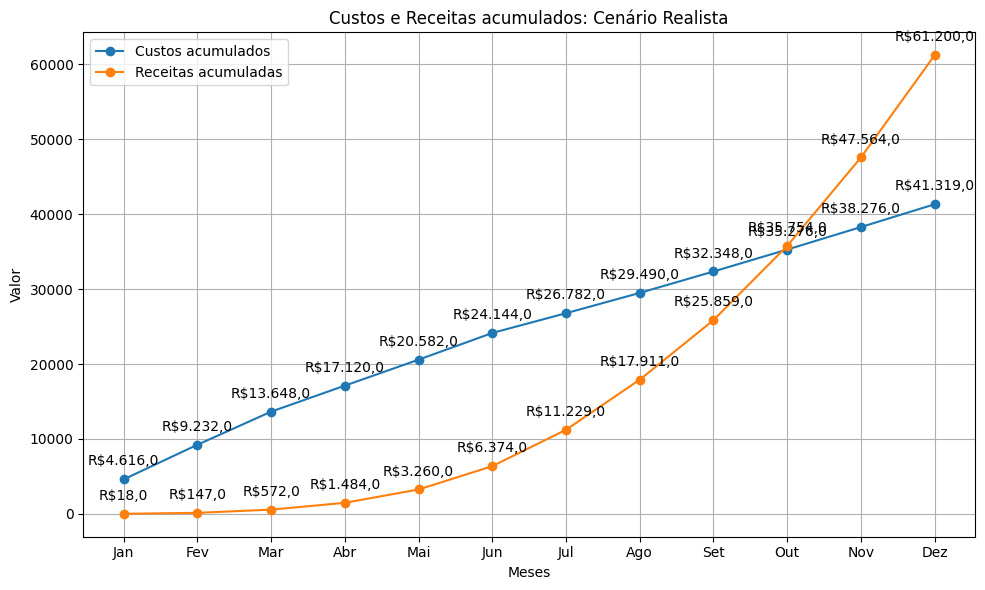
\includegraphics[scale=0.60]{imagens/viabilidadeFinanceira/Projeção-Receita_Custos-Realista.png}
    \label{cenarioRealista}
	\fonte{Os autores}
\end{figure}

\begin{figure}[H]
        \center
	\caption{\label{fig_sge20}Gráfico do Cenário Pessimista}
    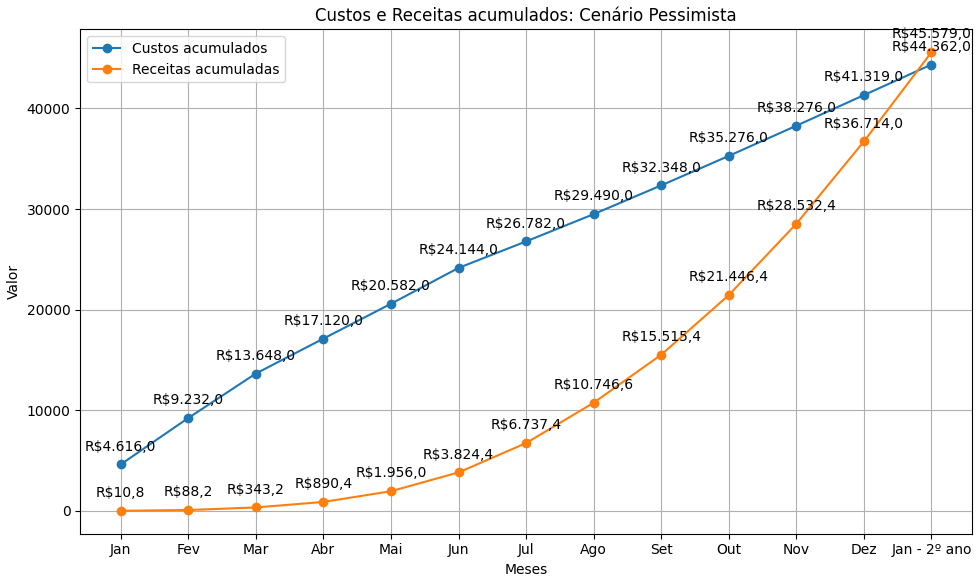
\includegraphics[scale=0.60]{imagens/viabilidadeFinanceira/Projeção-Receita_Custos-Pessimista.png}
    \label{cenarioPessimista}
	\fonte{Os autores}
\end{figure}

\begin{figure}[H]
        \center
	\caption{\label{fig_sge20}Gráfico do Cenário Otimista}
    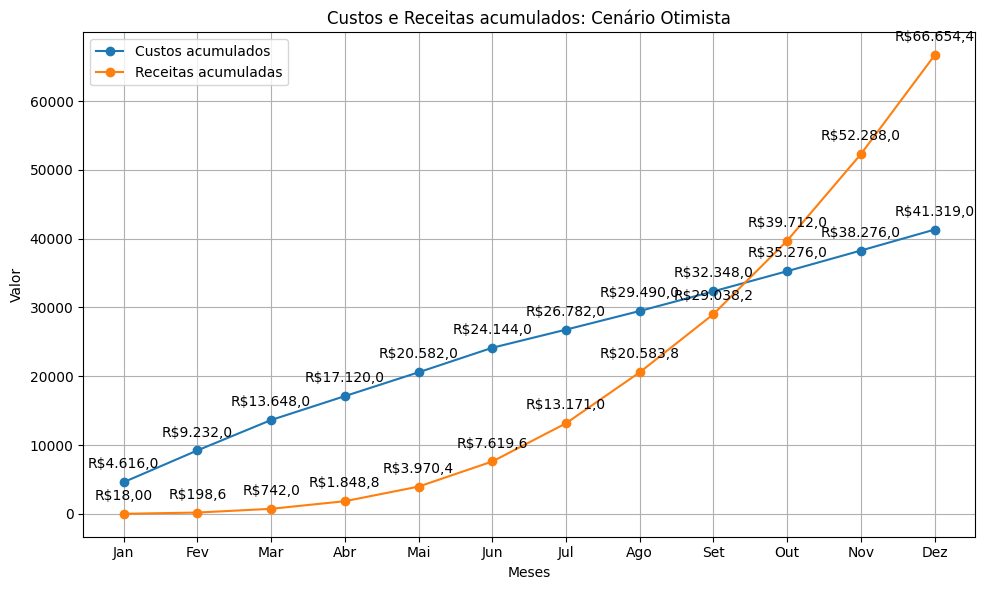
\includegraphics[scale=0.60]{imagens/viabilidadeFinanceira/Projeção-Receita_Custos-Otimista.png}
    \label{cenarioOtimista}
	\fonte{Os autores}
\end{figure}